\documentclass[aps,prl,reprint,amsmath,amssymb]{revtex4-1}

\usepackage{epsfig,color,graphicx}
%\usepackage{algorithmic}
\usepackage{algorithm}
\usepackage{algpseudocode}

% Mathematical symbols
\newcommand*{\imi}{i} % imaginary i
\newcommand*{\E}{\mathrm{e}}
% DIRAC NOTATION
% bra-ket vectors
\newcommand{\ket}[1]{\ensuremath{\vert #1 \rangle}}
\newcommand{\bra}[1]{\ensuremath{\langle #1 \vert}}
\newcommand{\braket}[2]{\ensuremath{\langle #1 \vert #2 \rangle}} % bra-ket inner product
\newcommand{\ketbra}[2]{\ensuremath{\vert #1 \rangle \langle #2 \vert}} % ket-bra outer product
% operators
\newcommand{\op}[1]{\ensuremath{\hat{#1}}} % operator
\newcommand{\opsb}[2]{\ensuremath{\hat{#1}_{#2}}} % operator with subscript
\newcommand{\opsp}[2]{\ensuremath{\hat{#1}^{#2}}} % operator with superscript

% left-right arrow with text above it
\makeatletter
\newcommand\xleftrightarrow[2][]{%
  \ext@arrow 9999{\longleftrightarrowfill@}{#1}{#2}}
\newcommand\longleftrightarrowfill@{%
  \arrowfill@\leftarrow\relbar\rightarrow}
\makeatother

% inexact differential
\def\dbar{{\mathchar'26\mkern-12mu d}}

%partial derivative with some variables held constant
\newcommand{\pdc}[3]{\ensuremath{\left( \frac{\partial #1}{\partial #2} \right)_{#3}}}
\newcommand{\pddc}[3]{\ensuremath{\left( \frac{{\partial}^2 {#1}}{\partial {#2}^2} \right)_{#3}}}

%average
\newcommand{\av}[1]{\ensuremath{\left\langle{#1}\right\rangle}} % operator

%text color
\newcommand{\new}{\color{red}}
\newcommand{\blue}{\color{blue}}
\newcommand{\old}{\color{black}}

\begin{document}

\bibliographystyle{apsrev}


\title{
Direct generalized and unconstrained localization of  one-electron orbitals
}

\author{Ziling Luo}
\email{ziling.luo@mail.mcgill.ca}
\author{Rustam Z. Khaliullin}
\email{rustam.khaliullin@mcgill.ca}
\affiliation{Department of Chemistry, McGill University, 801 Sherbrooke St. West, Montreal, QC H3A 0B8, Canada}

\date{\today}

\begin{abstract}
%RZZK: it is worth making the emphasis on the new approach to the localization procedure. Then say that, among other advantages, it is capable of producing more localized nonorthogonal orbitals.
Spatially localized molecular orbitals are of tremendous importance in electronic structure theory as they are widely used to describe chemical bonding and speed up calculations.
Nonorthogonal localized molecular orbitals (NLMOs) are known to be noticeably more localized than their conventional orthogonal counterparts. 
Unfortunately, the existing methods to obtain NLMOs must pre-determine and freeze the localization center of each NLMO before its spread is minimized. 
This is done to avoid the ``collapse'' of the occupied subspace – a problem of NLMOs becoming linearly dependent. 
In this paper, we describe an unconstrained black-box method to localize nonorthogonal orbitals that determines the position of their centers automatically during the optimization process. 
The key to the new procedure is to construct and impose a penalty function which prevents the orbital ``collapse''. 
An algorithm is proposed to adjust the strength of the penalty and produce the right balance between orthogonality and locality of NLMOs. 
The resulting method produces NLMO fast, without requiring any \emph{a priori} knowledge of bonding patterns in the system (i.e. ``chemical intuition'') and is demonstrated to work well a variety of molecules and materials (RZZK: gamma-point only) including large systems with non-trivial bonding. 
\end{abstract}

%RZZK: mention nonorthogonal maximally localized Wannier functions in the abstract

\maketitle

\section{Introduction} 

% RZZK: Potential reviewers: Weitao?, Marzari, LMO for CP2K developers.
% RZZK: borophene as a separate article?
% RZZK: should we do virtual states as well? No, let's leave them for the next paper.
% RZZK: Next paper can include virtual states (which will require preconditioning) and pipek-mezey localization functional

Spatially localized orbitals are of paramount importance in one-electron theories such as the Hartree-Fock (HF) method and Kohn-Sham density functional theory (DFT) as well as in post-HF wavefunction-based electron correlation methods.
Localized orbitals are widely used to describe and visualize chemical bonding between atoms thus helping classify bonds and understand electronic-structure origins of observed properties of atomistic systems~\cite{RZK}. 
Furthermore, localized orbitals are the key ingredient in multiple local electronic structure methods~\cite{goedecker1994efficient, bowler2012methods, zalesny2011linear, pulay1986orbital, saebo2001low, pisani2005local, hampel1996local, forner1997numerical} that dramatically reduce the computational cost of modeling electronic properties of large atomistic systems.~\cite{saebo1993local, schutz1999low, hetzer2000low, schutz2001low}
Spatially localized orbitals are known as localized molecular orbitals (LMOs) in the field of molecular quantum chemistry and maximally localized Wannier functions (MLWFs) in solid state physics and materials science. 
Here, they will be collectively referred to as LMOs whereas the eigenstates of the effective one-electron Hamiltonian will be called canonical molecular orbitals (CMOs) regardless of whether the system is isolated or treated with periodic boundary conditions.

%\bibitem{bowler2012methods}
%\bibinfo{author}{Bowler, D.} \& \bibinfo{author}{Miyazaki, T.}
%\newblock \bibinfo{title}{Methods in electronic structure calculations}.
%\newblock \emph{\bibinfo{journal}{Rep. Prog. Phys.}}
%  \textbf{\bibinfo{volume}{75}}, \bibinfo{pages}{036503}
%  (\bibinfo{year}{2012}).
%
%\bibitem{zalesny2011linear}
%\bibinfo{author}{Zale{\'s}ny, R.}, \bibinfo{author}{Papadopoulos, M.~G.},
%  \bibinfo{author}{Mezey, P.~G.} \& \bibinfo{author}{Leszczynski, J.}
%\newblock \emph{\bibinfo{title}{Linear-Scaling Techniques in Computational
%  Chemistry and Physics: Methods and Applications}}, vol.~\bibinfo{volume}{13}
%  (\bibinfo{publisher}{Springer Science \& Business Media},
%  \bibinfo{year}{2011}).

In traditional localization methods, LMOs are constructed by finding a unitary transformation of CMOs that minimizes a localization functional that effectively measures the spread of individual orbitals. 
Since CMOs are orthogonal and a unitary transformation preserves the overlap between orbitals, LMOs obtained in this way are orthogonal (OLMOs) by construction~\cite{weinstein1971localized}.
Multiple localization functionals have been proposed for molecular systems including Boys-Foster~\cite{boys1960construction}, Edmiston-Ruedenberg~\cite{bytautas2002electron, bytautas2003split, edmiston1963localized}, Pipek-Mezey~\cite{pipek1989a_fast}, and Von Niessen~\cite{niessen1972density}. For condensed phase periodic systems, RZK. ~\cite{marzari2012maximally}
%RZK: list and cite (reviews are preferred) appropriate localization methods (there should be one review by Nicola Marzari). 

Due to the imposed orthogonality condition, OLMOs exhibit small non-zero values even far away from the localization center. 
These orthogonalization tails complicate the interpretation of chemically relevant electronic-structure information and make its transferability from one system to another more difficult. More importantly, the tails reduce orbital locality making orbital-based local correlation methods less computationally efficient.
%
%RZK: I believe we can comment out the first approach as it is too different from the post-SCF methods that we describe here.
% To mitigate the undesirable orthogonality effects, it has been proposed to lift the orthogonality constraint during the localization procedure with the goal of increasing the flexibility and locality of LMOs. There are two distinct approaches to construct nonorthogonal LMOs (NLMOs). One approach bypasses CMOs and directly optimizes NLMOs that are constrained to a local space in the variational self-consistent filed (SCF) procedure~\cite{RZK}. Unfortunately, the localization constraints imposed on NLMOs can result in the NLMO energy being substantially higher than that of the fully delocalized state. Another approach is to obtain NLMOs is a post-SCF localization procedure that finds a nonsingular transformation of CMOs. 
% 
To mitigate the undesirable orthogonality effects, it has been proposed to replace a unitary transformation of CMOs with a more general nonsingular transformation. This generalization lifts the orthogonality constraint in the localization procedure and increases the number of degrees of freedom available to LMOs~\cite{anderson1968self, diner1968fully, magnasco1974localized, payne1977hartree, mehler1977self, feng2004An_efficient, cui2010efficient}. % RZK: I could have inadvetently used incorrect citations from your list. Please check. 
It has been found that NLMOs are indeed about $10-30 \%$ more localized than OLMOs if measured by the value of the Boys-Foster functional~\cite{feng2004An_efficient, liu2000nonorthogonal}. %(RZK: check whether the Boys-Foster functional is used indeed)  
% RZK the following (commented out) sentence is unclear: 
%The concept of NLMOs was first introduced by Anderson~\cite{anderson1968self} and Diner et al~\cite{diner1968fully} in 1968, but more efforts were devoted to constructing OLMOs previously.

Substantial recent efforts have been made to develop reliable algorithms to construct NLMOs~\cite{feng2004An_efficient, liu2000nonorthogonal, peng2013effective, hoyvik2017generalising}. % RZK: add citations for the a-priori methods?
%
Despite noticeable progress the existing methods produce NLMOs that are either still fairly similar to OLMOs [RZK: citation needed] or lead to the linear dependence between the orbitals~\cite{feng2004An_efficient}. 
%RZK I commented out this sentence because we rarily refer to the collapse. Perhaps we can call it linear dependence probelm throughout the paper: The latter problem is particularly widespread and will be referred to as the collapse problem. 
%RZZK: Strictly speaking the localization of nonorthogonal orbitals is an ill-defined problem because a global search for the minimum of the localization functional will yield an electronic state with all electrons ``collapsing into the single most localized orbital''
To overcome the widespread linear dependence problem, Yang and co-workers~\cite{feng2004An_efficient, cui2010efficient} have developed a localization method in which the centers of NLMOs are fixed during the minimization of the localization functional. 
The positions of the centers are predefined using those of the corresponding OLMOs~\cite{feng2004An_efficient} or simply guessed based on the knowledge of bonding patterns in a system~\cite{cui2010efficient}. %(i.e.``chemical intuition'')
While this method solves severe linear dependence issues, it requires either computational efforts to construct OLMOs centroids or good understanding of bonding properties in advance,which may limit the application of the method to relatively simple systems.

Out of several different localization schemes listed above, Boys-Foster localization functional~\cite{boys1960construction} is probably the most popular and commonly implemented.
In contract with Boys-Foster scheme, Pipek-Mezey method~\cite{pipek1989a_fast} does not mix between $\sigma$ and $\pi$ bonds, which helps to build a better understanding of the bonding pattern in the materials.
This scheme is based on maximizing the Mulliken charge~\cite{mulliken1955electronic} or L{\"o}wdin charge~\cite{lowdin1950non} of each orbital and guarantee that the $\sigma$-$\pi$ separation is always the stable solution compared with the mixed cases in OLMOs.


In this paper, we propose a direct and black-box method to construct LMOs, especially NOLMOs, that determines the optimal positions of their centers automatically in an unconstrained and straightforward optimization procedure, without \emph{a priori} knowledge of bonding patterns in the system.
In this new proposed method, we developed a generalize localization method  based on Boys-Foster and Pipek-Mezey scheme which allows users to control the orthogonality of the LMOs and select preferred localization schemes.
The key new component in the proposed method is a penalty function that prevents NLMOs from becoming linear dependent.
We present an algorithm for adjusting the penalty strength to find the desirable balance between the nonorthogonality and locality of LMOs. 
The localization method is demonstrated to work well for a variety of molecules and materials including large systems with non-trivial bonding. 

\section{Theory and algorithms}

The localization procedure starts with a set of occupied one-electron states $\ket{i_0}$. 
These orbitals are not assumed to be canonical or even orthogonal. 
However, they are assumed to be normalized, which does not reduce the generality of the method. 
Furthermore, the initial orbitals must be linear independent, that is, their overlap matrix $\sigma_{ji}^0 \equiv \braket{j_0}{i_0}$ must be invertible. 
The trial NLMOs are expressed as a linear combination of these initial states
%
\begin{equation}
\begin{split}
\ket{j} = \ket{i_0} {A^i}_j  
\end{split}
\end{equation}
%
The conventional tensor notation is used to work with the nonorthogonal orbitals~\cite{head1998tensor}: covariant quantities are denoted with subscripts, contravariant quantities with superscripts, and summation is implied over the same orbital indices.

The objective function minimized in this work contains two terms: a conventional localization functional $\Omega_L$ and a term that penalizes unphysical states with linearly dependent occupied orbitals $\Omega_P$:
%
\begin{equation} \label{eq:fun-pen}
\begin{split}
\Omega(\mathbf{A}) = \Omega_L(\mathbf{A}) + c_P \Omega_P(\mathbf{A}), \\
\Omega_P(\mathbf{A}) = - \log \det \left[ \sigma (\mathbf{A}) \right]
\end{split}
\end{equation}
%
where $c_P > 0$ is the penalty strength, $\sigma$ is the NLMO overlap matrix 
%
\begin{equation}
\begin{split}
\sigma_{kl} = \braket{k}{l} = {A^j}_k \sigma_{ji}^0{A^i}_l
%= (\mathbf{A}^\dagger \mathbf{T}^\dagger \mathbf{ S T A})_{kl},
\end{split}
\end{equation}
%

\begin{figure}[H]
\begin{algorithm}[H]
  \caption{Conjugate gradient minimization of $\Omega$}
  \label{alg:cg}
   \begin{algorithmic}[1]
   	%\Procedure{Minimize$\Omega$}{$c_P, \tau, \mathbf{T}_0$}
	\State Input $\epsilon_{\text{CG}}$ \Comment{Localization convergence threshold}
	%\State Input $N_{\text{CG}}$, $N_{\text{Outer}}$ \Comment{Max CG, outer iterations}
	\State Input $\text{D}_{\text{min}}$ \Comment{Minimum allowed NLMO determinant}
   	\State Input $\mathbf{T}_0$ \Comment{Initial basis set coefficients for $\ket{i_0}$}
   	\State Input $\mathbf{S}$ \Comment{Basis set overlap}
   	\State Input $\mathbf{L}^K$ \Comment{Basis set representation of the localization operator} 
   	\State $\mathbf{\sigma}_0 \gets \mathbf{T}_0^{\dagger} \mathbf{ST}_0$ \Comment{Initial orbital overlap} 
   	\State $\mathbf{B}^{K} \gets \mathbf{T}_0^{\dagger} \mathbf{L}^K \mathbf{T}_0$ \Comment{Initial localization matrix, Eq.~(\ref{eq:fun-loc})} 
	\State $\mathbf{a} \gets \mathbf{I}$ \Comment{Initial guess on variational parameters}
	%\State Converged $\gets$ False
	\State StopOuter $\gets$ False \Comment{Flag to exit the outer loop}
	\State $i_{\text{Outer}} \gets 0$ \Comment{Iteration counter}
	\Repeat \Comment{Loop to change the penalty strength}
		\State $i_{\text{Outer}} \gets i_{\text{Outer}} + 1$ 
		\State StopCG $\gets$ False \Comment{Flag to exit the CG loop}
		\State $i_{\text{CG}} \gets 0$ \Comment{Iteration counter}
%		\State $\beta \gets 0$ \Comment{Reset conjugation}
		\Repeat \Comment{Fixed-penalty localization loop}
			\State $i_{\text{CG}} \gets i_{\text{CG}} + 1$ 
			\State $\mathbf{A} \gets \mathbf{a} \left[ \text{diagonal}(\mathbf{a}^{\dagger} \mathbf{\sigma}_0 \mathbf{a}) \right]^{-\frac{1}{2}}$ \Comment{Update NLMOs}
			\State $\mathbf{\sigma} \gets \mathbf{A}^{\dagger}\mathbf{\sigma}_0 \mathbf{A}$ \Comment{Update overlap}
			\State $\text{Det} \gets \text{determinant} (\mathbf{\sigma})$ \Comment{Determinant}
			\State $\Omega_{P} \gets - \log [\text{Det}] $ \Comment{Orthogonalization functional}
			\State $\mathbf{P} \gets \text{Eq~(\ref{eq:grad-pen}) and~(\ref{eq:grad-convert})}$ \Comment{Orthogonalization gradient}
			\State $\Omega_{L} \gets \text{Eq~(\ref{eq:fun-loc})}$ \Comment{Localization functional}
			\State $\mathbf{L} \gets \text{Eq~(\ref{eq:grad-loc}) and~(\ref{eq:grad-convert})}$ \Comment{Localization gradient}
			\If{$i_{\text{Outer}}=1$ \textbf{and} $i_{\text{CG}}=1$} 
				%\State $c_{P} \gets \text{Tr}(\mathbf{L}^{\dagger} \mathbf{P})/\text{Tr}(\mathbf{P}^{\dagger}\mathbf{P})$
				\State $c_{P} \gets \Omega_{L}(\log [\text{Det} / \text{D}_{\text{min}} ])^{-1}$ \Comment{Initial strength}
			\EndIf
			\State $\Omega \gets \Omega_{L} + c_P \Omega_{P} $ 
			\If{$i_{\text{CG}}>1$}
				\State $\mathbf{\Gamma} \gets \mathbf{G}$ \Comment{Save old gradient}
			\EndIf 
			\State $\mathbf{G} \gets \mathbf{L} + c_P \mathbf{P} $ 
			%\State $\text{Error}_\text{CG} \gets \vert\vert \mathbf{G} \vert \vert_{\text{max}}$
			\If{$\vert\vert \mathbf{G} \vert \vert_{\text{max}} < \epsilon_{\text{CG}}$}
				\State StopCG $\gets$ True
			\EndIf
%			\If{$i_{\text{CG}}=1$ \textbf{And} $i_{\text{Outer}}=1$}
%				\State StopCG $\gets$ False \Comment{Do first iteration}
%			\EndIf
			\If{\textbf{not} StopCG}
%				\If{$i_{\text{CG}} = 1$}
%					\State $\mathbf{P}^{R_c} \gets \text{Eq.\ref{eq:prec}}(\mathbf{F},\mathbf{M}^{R_c},\mathbf{K}^{R_c}) $\Comment{Precon.}
%				\Else
%					\State $\mathbf{O}_{R_c} \gets \mathbf{D}_{R_c}$ \Comment{Save old direction}
%				\EndIf
				\If{$i_{\text{CG}} > 1$}
					\State $\mathbf{O} \gets \mathbf{D}$ \Comment{Save old direction}
				\EndIf
%				\State $\mathbf{D}_{R_c} \gets - [(\mathbf{P}^{R_c})^{-1} \mathbf{G}^{R_c}]_{R_c}$ \Comment{Precon. grad.}
				\State $\mathbf{D} \gets - \mathbf{G}$ \Comment{Initial direction}
				\If{$i_{\text{CG}}>1$}
					\State $\beta \gets \text{Tr}(\mathbf{G}^{\dagger} \mathbf{D})/\text{Tr}(\mathbf{\Gamma}^{\dagger}\mathbf{O})$
					\State $\mathbf{D} \gets \mathbf{D} + \beta \mathbf{O}$ \Comment{Search direction}
				\EndIf 
				\State $\alpha \gets \text{argmin}_{\alpha} \Omega(\mathbf{a} + \alpha \mathbf{D})$ \Comment{Line search}
				\State $\mathbf{a}\gets \mathbf{a} + \alpha \mathbf{D}$ \Comment{Update variational DOFs}
			\EndIf
		\Until{StopCG} 
%RZK: add an additional criterion that prevents high-determinant cases go on forever
		%\If{$\text{Det} < \text{Det}_{\text{Target}}$ \textbf{or} $i_{\text{Outer}} > N_{\text{Outer}}$}
		\If{$\text{Det} < \text{D}_{\text{min}}$}
			\State StopOuter $\gets$ True
		\EndIf
		\If{$i_{\text{Outer}}>1$} 
			\State $c_{P} \gets c_P / 2$ \Comment{Reduce $c_P$}
		\EndIf
	\Until{StopOuter}
	\State $\mathbf{return}$ $\mathbf{T} \gets \mathbf{T}_0 \mathbf{A} $ \Comment{Return NLMOs coefficients}
	%\EndProcedure
   \end{algorithmic}
\end{algorithm}
\caption{\label{fig:cg} Algorithm for the optimization of NLMOs.}
\end{figure}

If the NLMOs are normalized the determinant of $\sigma$ varies from 1 for orthogonal NLMOs to 0 for linearly dependent NLMOs. The penalty function---the key ingredient of the proposed method---varies from 0 to $+\infty$ for these two extreme cases, making linearly dependent state inaccessible in the localization procedure with finite penalty strength $c_P$. 
% RZZK: Why sigma instead of A? quadratic penalty in terms of A (more complicated in terms of a). Why log?
A normalization constraint can be imposed on NLMOs if their coefficients are expressed in terms of independent variational parameters denoted with lowercase $\mathbf{a}$
%
\begin{equation}
\begin{split}
{A^i}_j = {a^i}_{j} ({a^k}_{j} \sigma^0_{kl}{a^l}_{j})^{-\frac{1}{2}} \equiv {a^i}_{j} N_j ,
\end{split}
\end{equation}
%
where the $\mathbf{a}$-dependent normalization coefficient $N_j$ is defined for brevity. 

The inclusion of the penalty term converts the localization procedure into an unconstrained and straightforward optimization problem. Additionally, adjusting the strength of the penalty $c_P$ enables one to achieve the right balance between the nonorthogonality and locality of the orbitals (see below). 

In this work, we adopted the localization functional proposed by Resta~\cite{resta1998quantum, resta1999electron} and generalized by Berghold \emph{et al.}~\cite{berghold2000general} to three dimensions and simulation cells of general shape and symmetry: 
% RZK: 
% berghold2000general --- PHYSICAL REVIEW B, 61, 10040
% resta1999electron https://doi.org/10.1103/PhysRevLett.82.370
% resta1998quantum -- Phys. Rev. Lett. 80, 1800 (https://doi.org/10.1103/PhysRevLett.80.1800)
% silvestrelli1999maximally -- PRB 59 9703
%
% RZK: do we really use log function? If not, fix the gradient (PM and Boys are consistent then) and re-write the PM section to include only the kernel instead of all three equation (alpha->K). If yes, the PM gradient must be different.
\begin{equation} \label{eq:fun-loc}
\begin{split}
\Omega_L(\mathbf{A}) &= - \sum_K \sum_i \omega_K \log \vert z_{i}^{K} \vert^2, \\
z_{i}^{K} &= {A^m}_i B^{K}_{mn} {A^n}_i, \\
B^{K}_{mn} &= \bra{m_0} \E^{\imi \mathbf{G}_K \cdot \mathbf{\op{r}}} \ket{n_0}
\end{split}
\end{equation}
%
where $\mathbf{\op{r}}$ is the position operator in three dimensions, $\omega_K$ and $\mathbf{G}_K$ are a suitable set of weights and reciprocal lattice vectors, respectively, labeled by index $K$~\cite{silvestrelli1999maximally, berghold2000general}. We chose to write the summation over $K$ explicitly because $K$ is not an orbital index. The functional in Eq.~(\ref{eq:fun-loc}) can be used for both gas-phase and periodic systems~\cite{berghold2000general}. In the former case, the functional is equivalent to the Boys-Foster localization~\cite{berghold2000general, resta1999electron}. In the latter case, its applicability is limited to the electronic states described within the $\Gamma$-point approximation.

We also considered the Pipek-Mezey localization functional~\cite{pipek1989fast,lehtola2014pipek} that has the advantage of preserving the separation of $\sigma$ and $\pi$ bonds and is commonly employed for molecular system
%RZK citation lehtola2014pipek: dx.doi.org/10.1021/ct401016x
%RZK citation pipek1989fast: Pipek, J.; Mezey, P. G. J. Chem. Phys. 1989, 90, 4916 
%
\begin{equation} \label{eq:pipek}
\begin{split}
\Omega_L^{\text{PM}}(\mathbf{A}) &= - \sum_{\alpha=1}^{\text{Atoms}} \sum_i \vert z_{i}^{\alpha} \vert^2, \\
z_{i}^{\alpha} &= {A^m}_i B^{\alpha}_{mn} {A^n}_i, \\
B^{\alpha}_{mn} &= \frac{1}{2} \sum_{\mu \in \alpha} \bra{m_0}  \left( \ketbra{\chi_{\mu}}{\chi^{\mu}} + \ketbra{\chi^{\mu}}{\chi_{\mu}} \right) \ket{n_0}
%RZZK alpha and mu do not belong to the same set
\end{split}
\end{equation}
%
%
where $z_{i}^{\alpha}$ is the contribution of orbital $i$ to the Mulliken charge of atom $\alpha$, $\ket{\chi_\mu}$ and $\ket{\chi^\mu}$ are atom-centered covariant and contravariant basis set functions~\cite{silvestrelli1999maximally, berghold2000general}. The summation over $\mu$ is written explicitly to emphasize that it is restricted to the basis functions centered on atom $\alpha$. 

%RZZK: PM discussion

The unconstrained minimization of functional $\Omega$ with fixed $c_P$ can be carried out with a variety of algorithms. In this work, we used a simple conjugate gradient algorithm summarized in Figure~\ref{fig:cg}. The gradient ${G_i}^j \equiv \frac{\partial \Omega}{\partial {a^i}_j}$  required in the algorithm is a sum of the localization ${L_i}^j \equiv \frac{\partial \Omega_L}{\partial {a^i}_j}$ and penalty ${P_i}^j \equiv \frac{\partial \Omega_P}{\partial {a^i}_j}$ components
%
\begin{equation} \label{eq:grad}
\begin{split}
G{_k}^{l} = L{_k}^{l} + c_P P{_k}^{l}.
\end{split}
\end{equation}
%
These components can be readily expressed in terms of the derivatives with respect to the transformation coefficients $\tilde{X}{_k}^l \equiv \frac{\partial \Omega_X}{\partial {A^k}_l}$, where $X$ is either $L$ or $P$:
%
\begin{equation} \label{eq:grad-convert}
\begin{split}
{X_i}^j & = \tilde{X}{_k}^l \frac{\partial {A^k}_l}{\partial {a^i}_j} = \left[ \tilde{X}{_i}^j - ( \sigma_{in}^0 {A^n}_j ) ( {A^m}_j \tilde{X}{_m}^j ) \right] N_j 
\end{split}
\end{equation}
%
\begin{equation} \label{eq:grad-loc}
\begin{split}
\tilde{L}{_k}^l & = - \sum_K \frac{4 \omega_K}{\vert z_{l}^{K} \vert^2} \times \\ 
&\times \left[  \operatorname{Re}(B^{K}_{kn}) {A^{n}}_{l} \operatorname{Re}(z_{l}^{K}) + \operatorname{Im}(B^{K}_{kn}) {A^{n}}_{l} \operatorname{Im}(z_{l}^{K}) \right]
\end{split}
\end{equation}
%
\begin{equation} \label{eq:grad-pen}
\begin{split}
\tilde{P}{_k}^l & = -2 \sigma_{km}^0 {A^m}_n \sigma^{nl} 
\end{split}
\end{equation}
%

\textbf{Penalty strength.} If the penalty strength $c_P$ is extremely large, $\Omega_L$ is negligible compared to the penalty term and the minimization of $\Omega$ is numerically equivalent to a trivial orbital orthogonalization. In the opposite case of extremely small $c_P$, the minimization of $\Omega$ may result in a linear dependence between NLMOs as reported earlier~\cite{cui2010efficient}. % RZK: cite Weitao's paper, in which they fix centroids.
In the latter case, the algorithm shown in Figure~\ref{fig:cg} fails to compute the inverse of the NLMO overlap required in Eq.~(\ref{eq:grad-pen}). 

As we show below, there is a wide range of $c_P$ values between the two extremes that produce NLMOs that are substantially more localized than OLMOs and linearly independent.  
Within this range, $c_P$ serves as an adjustable parameter that can be used to achieve a desirable locality-orthogonality compromise. 
For a fixed value of $c_P$, the degree of linear dependence between the optimal NLMOs can be measured by the value of the determinant of the NLMO overlap matrix. 
Thus, the flexibility of the penalized localization method presented here can be favorably compared to the existing methods that produce either orthogonal orbitals, linearly-dependent LMOs, or NLMOs with fixed localization centers. 

A simple strategy to find an appropriate penalty strength is to minimize $\Omega$ with a sufficiently large initial $c_P$ value and then gradually decrease $c_P$ until the determinant of the overlap of the \emph{optimal} NLMOs drops below a desired threshold $\text{D}_{\text{min}} \in (0,1]$. 
The initial value of $c_P$ should be chosen to balance approximately the localization and penalty components of $\Omega$. 
Thus, a reasonable initial value of $c_P$ can be estimated by assuming that the reduction in $\Omega_L$ upon the minimization of $\Omega$ has the same order of magnitude as the change in the penalty $c_P \Omega_P$:
%
\begin{equation} \label{eq:cp-beta}
\begin{split} 
%\Omega_L(\mathbf{I}) + c_P \Omega_P(\mathbf{I}) & \sim \Omega_{L}(\mathbf{A}^{\ast}) - c_P \log \text{D}_{\text{min}} \\
c_P^{\text{init}} & \sim \frac{ \Omega_{L}(\mathbf{I}) - \Omega_{L}(\mathbf{A}^{\ast}) }{ \Omega_{P}(\mathbf{A}^{\ast}) - \Omega_{P}(\mathbf{I}) } = \frac{ \beta_L^{\ast} }{ \beta_P^{\ast} } \times \Omega_{L}(\mathbf{I})
\end{split}
\end{equation}
%
where $\mathbf{A}^{\ast}$ denotes the (yet unknown) solution to the minimization problem, 
%
\begin{equation} 
\begin{split} 
\beta_L^{\ast} \equiv \frac{\Omega_L(\mathbf{I})- \Omega_L(\mathbf{A}^{\ast})}{\Omega_L(\mathbf{I})} \in [0,1]
\end{split}
\end{equation}
%
is the (positive) expected relative reduction in the localization functional, and 
%
\begin{equation} \label{eq:betap}
\begin{split} 
\beta_P^{\ast} \equiv \log \frac{\det \sigma(\mathbf{I})}{ \det \sigma(\mathbf{A}^{\ast}) } \approx \log \frac{\det \sigma(\mathbf{I})}{ \text{D}_{\text{min}} } \equiv \beta_P > 0
\end{split}
\end{equation}
%
is the logarithm of the ratio of the initial and final determinants. 
The importance of Eqs.~(\ref{eq:cp-beta})--(\ref{eq:betap}) is that they allow to estimate the initial value of $c_P$ as $\Omega_L(\mathbf{I})$, which can be easily calculated in the beginning of the optimization procedure, multiplied by a dimensionless constant $\alpha$
%
\begin{equation} \label{eq:cp-alpha}
\begin{split}
c_{P}^{\text{init}} = \frac{ \beta_L^{\ast} }{ \beta_P } \times \Omega_L(\mathbf{I}) \equiv \alpha \times \Omega_L(\mathbf{I})
\end{split}
\end{equation}
%
Eq.~(\ref{eq:cp-alpha}) makes clear that the penalty component is an extensive function of a system with the units that are consistent with the localization component. Although the optimal dimensionless parameter $\beta_L^{\ast}$ is not known \emph{a priori} its magnitude can be easily estimated to obtain a sufficiently large initial guess for $c_P$. For example, an optimization of canonical orbitals $\det \sigma(\mathbf{I})=1$ that stops when the NLMO determinant drops below $\text{D}_{\text{min}} = 0.1$ can be initialized by adopting the maximum possible value of $\beta_L^{\ast} = 1$ that results in $\alpha = \log^{-1} 10$.

The procedure for tuning $c_P$ is shown as the outer loop of the algorithm in Figure~\ref{fig:cg}. Its only required input is $\text{D}_{\text{min}}$. % Parameter $\alph$ is then computed using Eq.~(\ref{eq:cp-alpha}). Alternatively, parameter $\alpha$ can be specified as an input. It is also %RZZK

%RZZK: Depending on the results discuss the following: If the precise value of the determinant is necessary the penalty can be replaced with c_P becoming a Langrange multiplier that can be determined precisely. In a MD or geopt, determine $c_P$ once and then fix it for subsequent geometries. This is valid as long as the electronic properties of the system remain the same (e.g. there is not insulator to metal phase transition). 

%RZZK: Dmin is a misnomer.

%RZZK: Describe the procedure for quick and reliable determinant evaluation

\section{Computational details}

The localization procedure is implemented in the CP2K software package~\cite{cp2kgeneral}. 
We constructed NLMOs for several systems ranging from a simple water molecule to complex molecules with non-trivial bonding patterns to large periodic systems. 
CMOs were obtained for all systems using the conventional SCF procedure in the DFT module of CP2K and then used as the initial states in the localization procedure. 
The Becke-Lee-Yang-Parr generalized gradient approximation~\cite{becke1988density, lee1988development} was used as the exchange-correlation functional.
Goedecker-Teter-Hutter pseudopotentials~\cite{goedecker1996separable} were used together with a triple-$\zeta$ atom-centered Gaussian basis set with two sets of polarization functions for all atoms. 
The energy cutoff of 600 Ry 
%(RZK: if we need to redo the calculation increase the energy cutoff to 300Ry) 
was used to define the auxiliary plane-wave basis set in the construction of the effective Hamiltonian. 
The integration over the Brillouin zone was performed using the single $\Gamma$ point.

%RZK: If all systems use the same optimization parameters list them in this section. If parameters are different, we need to discuss how we tune them in the Results and discussion.

\section{Results and discussion}

% RZK: The plan is:
%*** Demonstrate how the penalty-strength algorithm works with the default and user-specified input parameters: $\alpha$, D$_{\text{min}}$, reduction factor. For selected, illustrative examples present figures showing optimal NLMO localization and determinant as a function of $c_P$.
%*** Compare the spread (what do we use as the spread proxy?) of CMOs, OLMOs, NLMOs for simple systems. The main question is whether relaxation of the centroid position allows to achieve better localization. Perhaps not. 
%*** Demonstrate that the new scheme reproduces the expected localization on bonds. Show graphene example.
%*** Show how the new scheme works for more complex systems. Borans and carboranes.
%*** Illustrate reduction in the orthogonalization tails.
%*** Anything else?

%we compared the performance of the newly developed method to the traditional localization that generate OLMOs and previously reported NLMO methods. 

% RZK: report percentages obtained with the previous method. 
% RZK: I do not think we need absolute values of the localization functioal.
% RZK: use beta values defined in the equations above instead of percentage redaction, a priori and posteriori values of alpha

\begin{table*}[htbp]
\caption{The localization functional, final determinant and relative percentage of NLMOs compared with OLMOs.}
\label{tab:loc}
\centering
\begin{tabular}{l c c c c}
\hline\hline
Molecules & $\Delta_{\text{OLMOs/CMOs}}$  & $\Delta_{\text{NLMOs/CMOs}}$ & $\Delta_{\text{NLMOs/OLMOs}}$ & $\det(\sigma)$ \\
\hline
H$_2$O & 0.221 & 0.364 & 0.183 & 0.100 \\ 
CO$_2$ & 0.650 & 0.755 & 0.302 & 0.025 \\
Diborane (B$_2$H$_6$) & 0.617 & 0.640 & 0.062 & 0.745 \\
Borazine (B$_3$N$_3$H$_6$) & 0.726 & 0.781 & 0.202 & 0.026 \\
Carborane (C$_2$B$_{10}$H$_{12}$) & 0.717 & 0.764 & 0.166 & 0.085 \\ 
Propene (C$_3$H$_6$) & 0.609 & 0.665 & 0.143 & 0.042 \\
1-Butyne (C$_4$H$_6$) & 0.624 & 0.696 & 0.193 & 0.063 \\
Benzene (C$_6$H$_6$) & 0.694 & 0.779 & 0.278 & 0.041 \\ 
Heptane (C$_7$H$_{16}$) & 0.889 & 0.902 & 0.120 & 0.122 \\ 
Icosane (C$_{20}$H$_{42}$) & 0.975 & 0.978 & 0.112 & 0.053 \\ 
Decacyclene (C$_{72}$H$_{24}$) & 0.935 & 0.947 & 0.161 & 0.042 \\ 
Graphene & 0.769 & 0.816 & 0.205 & 0.025 \\
\hline
Average & 0.702 & 0.757 & 0.179 & 0.114 \\
\hline
\hline
\end{tabular}
\label{table:nonlin}
%RZK: report $\text{D}_{\text{min}}$ in the footnote
\end{table*}

% (H$_2$O, CO$_2$, C$_3$H$_6$, C$_4$H$_6$, B$_2$H$_6$, B$_3$N$_3$H$_6$, C$_6$H$_6$, C$_7$H$_{16}$, C$_2$B$_{10}$H$_{12}$, C$_{20}$H$_{42}$, C$_{72}$H$_{24}$, graphene). 
%RZK: Do you think the reader will understand what systems you describe based only on their chemical formulas? All systems must be properly named and described in sufficient detail so the reader know what molecule you are talking about.

% RZK: The graphs are of poor quality, line styles must be changed. What points are we going to include? They must be in agreement with our $c_P$ adjustment algorithm.
% RZK: We do not need Max determinant because the position of the line is obvious.
% RZK: We need to reference the algortihm used for OLMO localization because the OLMO line is higher than the maximum in our line.

\begin{figure*}[hbpt]
\centering
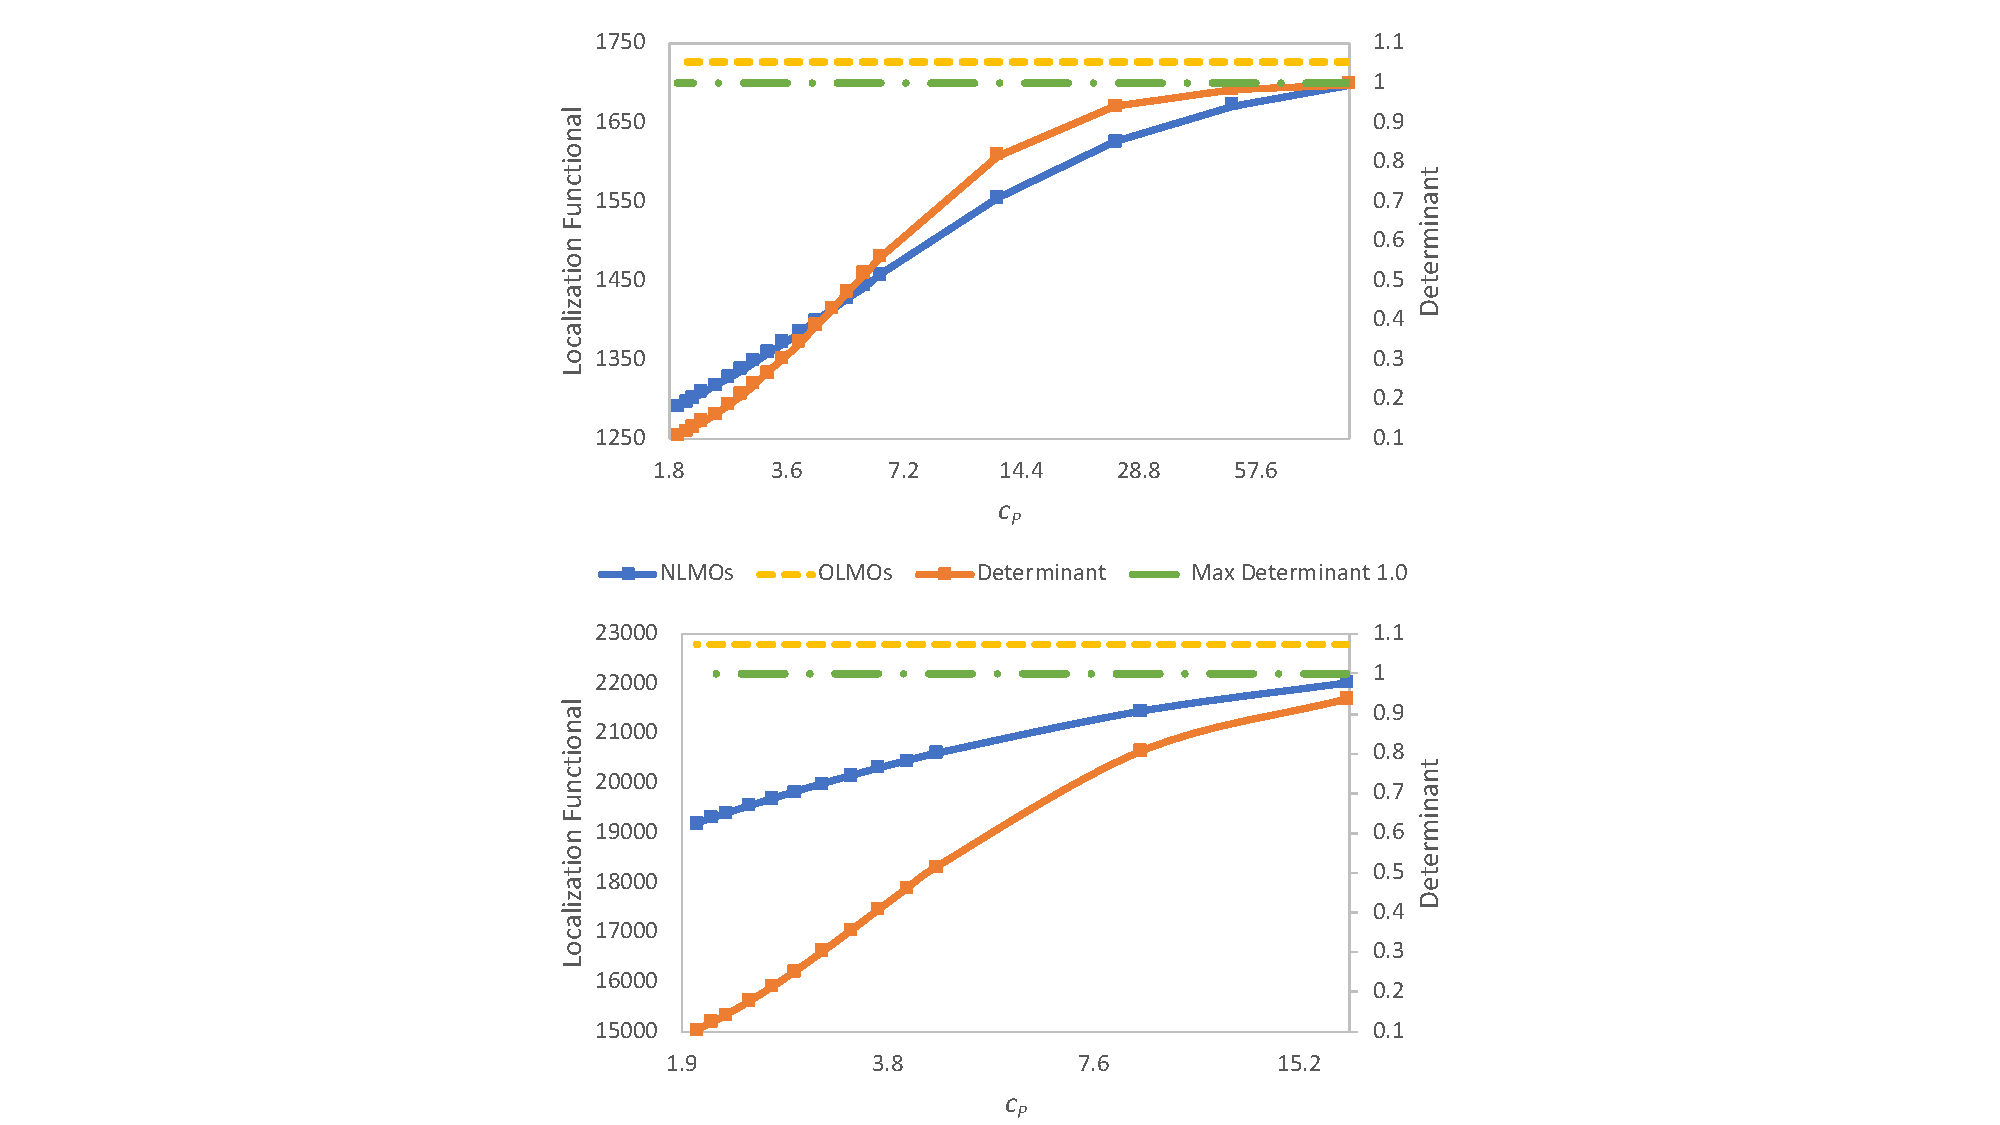
\includegraphics[width=\textwidth]{figure_2.pdf}
\caption{The dependence of the localization functional and determinant of NLMO overlap on $\alpha$ -- the adjustable part of the penalty strength.}
\label{fig:alpha}
\end{figure*}

%RZK: do not use table/figure numbers directly. Use \ref, as I demostrated above. 

Among all of our tested systems, the optimization procedure is stable and efficient based on the conjugate gradient method. 
To illustrate the extent and orthogonality of the final localized MOs, the Berghold functionals ~\cite{berghold2000general}  are calculated to compare the difference between CMOs, OLMOs and NLMOs.
The results are shown in the Table~\ref{tab:loc}.
The determinants controlled by the penalty strength $\alpha$ and final determinant cutoff are listd in the last column of Table~\ref{tab:loc} from all systems, which also indicate the orthogonality of the obtained NLMOs.
Even though the final determinant could go down to extremely small value (such as $10^{-7}$) in some systems, we set 0.02 a.u. as the final determinant cutoff since we suspect some generated NLMOs may become linear dependent with those extremely small determinant values.
So we dismiss all generated NLMOs with final determinant less than 0.02 a.u. to prevent orbitals from collapsing.
The final determinant value and further visual detection have shown that all final obtained NLMOs are linear independent between each other.

Yang et al.~\cite{feng2004An_efficient, cui2010efficient} have proved that, the NLMOs are more compact than the corresponding OLMOs with about $10\%$ to $30\%$ in the value of spread functional based on their prefixed centers algorithms.
Our algorithms gave the similar results with theirs.
The relative decreases of the localization functions of the OLMOs to CMOs, NLMOs to CMOs and NLMOs to OLMOs are tabulated in the columns of 2-4 of Table~\ref{tab:loc}, respectively.
The relative decrease of OLMOs compared with CMOs is range from 0.221 to 0.975 and the NLMOs are further  more localized, which are 0.364 to 0.978 more compact to the CMOs.
The average  localization functional decreases of OLMOs and NLMOs to CMOs are 0.702 and 0.757.
Comparison between the NLMOs and OLMOs based on our algorithms gives similar results with previous study, which the NLMOs are 0.062 to 0.302 more localized to the OLMOs, with 0.179 in average.

%RZK: Move to restuls. Discuss why this threshold is taken. 

The relationships between $\alpha$ and localization functional and determinant are illustrated in the Figure~\ref{fig:alpha} with the initial suggested penalty strength ($\alpha = \log^{-1} 10$) as the initial point.
The reason of using suggested $\alpha$ as starting point is that we do observe the scenario described in the Theory section, which results in the case that the negligible localization functional and a trivial orbital orthogonalization problem may be encountered when using extremely large penalty strength at the beginning of the optimization.
The first vertical axis and the red line describe the change of localization functional with different penalty strength during the minimization procedure, with the secondary axis and the blue line report the variation of determinants.
The trend of the localization functional and determinant versus penalty strength change in the same way as we expected.
For most of the systems such as propene, graphene and benzene, the suggested $\alpha$ directly helps users to eliminate the  negligible localization functional problem even in the first several steps.  
But we still got a typical dependency results in the Heptane system, which we observe both localization functional and determinants remain the same for the first and last several points and change relatively faster in the middle points.
The resulting figure of Heptane suggests that our initial suggested penalty strength help avoiding the long term trivial orbital orthogonalization problem for the beginning period.
According to the Figure~\ref{fig:alpha}, we can conclude that our method successfully generate fast and reliable linear independent NLMOs based on the black-box algorithm.

\begin{figure*}[hbpt]
\centering
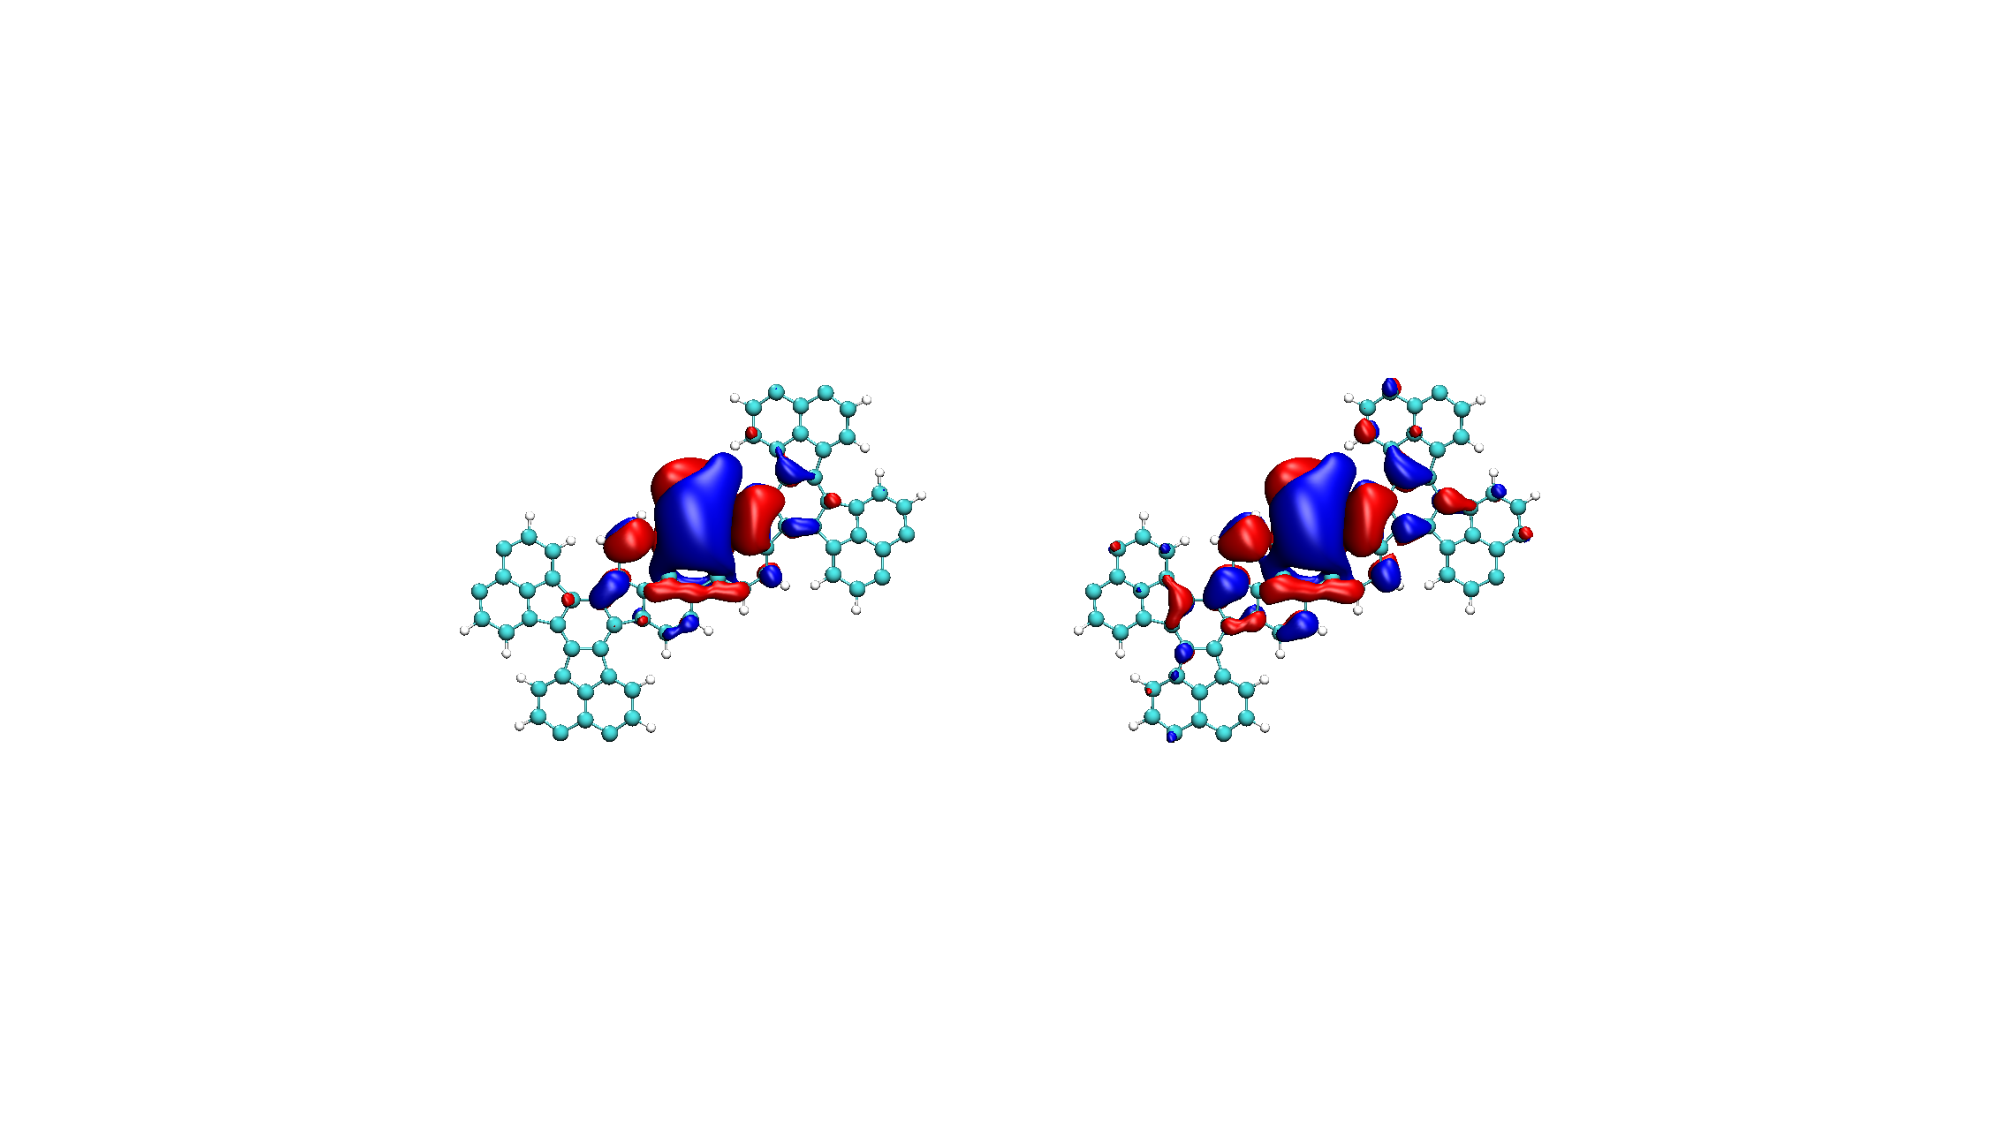
\includegraphics[scale=0.5]{figure_3.pdf}
\caption{A plot of the OLMO and NLMO of the covalent bond of adjacent carbon atoms with different view direction  in C$_2$B$_{10}$H$_{12}$ molecule. (isosurface value eauqls to 0.04~a.u.)}
\label{fig:boro}
\end{figure*}

%RZK: remove grpahene image. Draw the periodic cell on one of the images. Same for the Zhenzhe's polymer.
\begin{figure*}[hbpt]
\centering
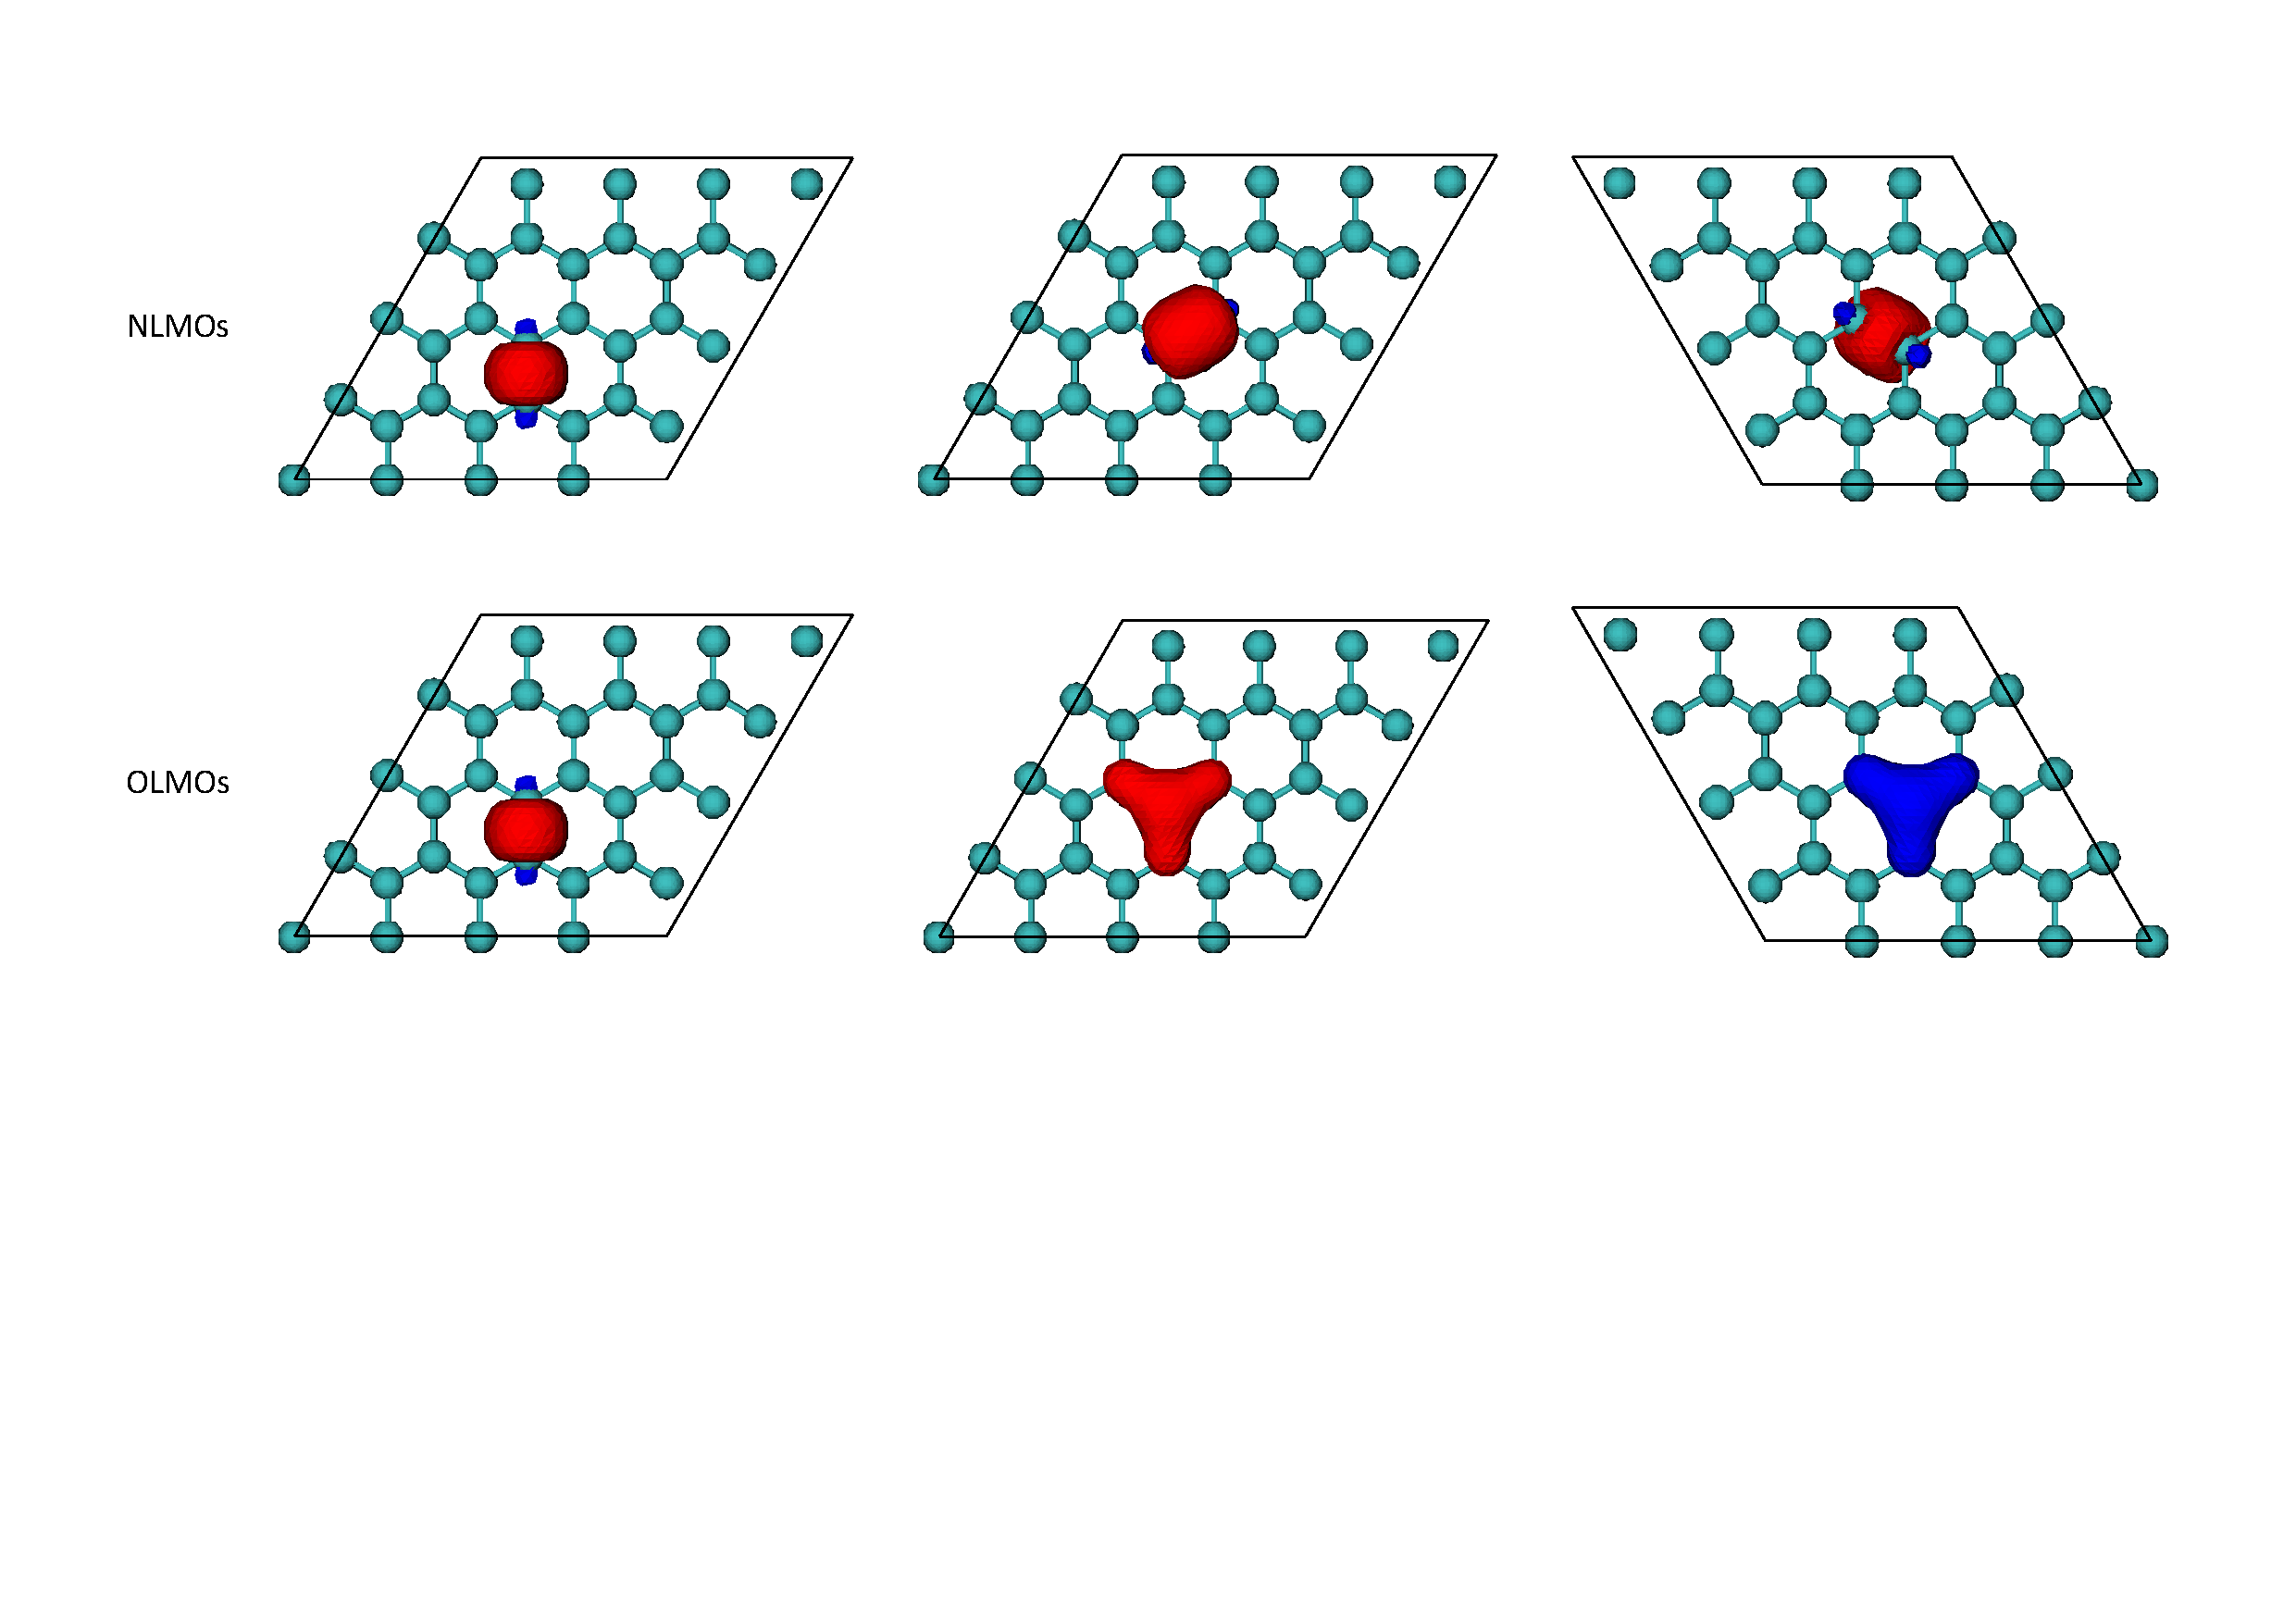
\includegraphics[scale=0.5]{figure_4.pdf}
\caption{A plot of the OLMO and NLMO of the $\sigma$ bond~(second column) and $\pi$ bond~(third and forth column) in graphene. (isosurface value equals to  0.06~a.u.)}
\label{fig:graphene}
\end{figure*}

\begin{figure*}[htbp]
\centering
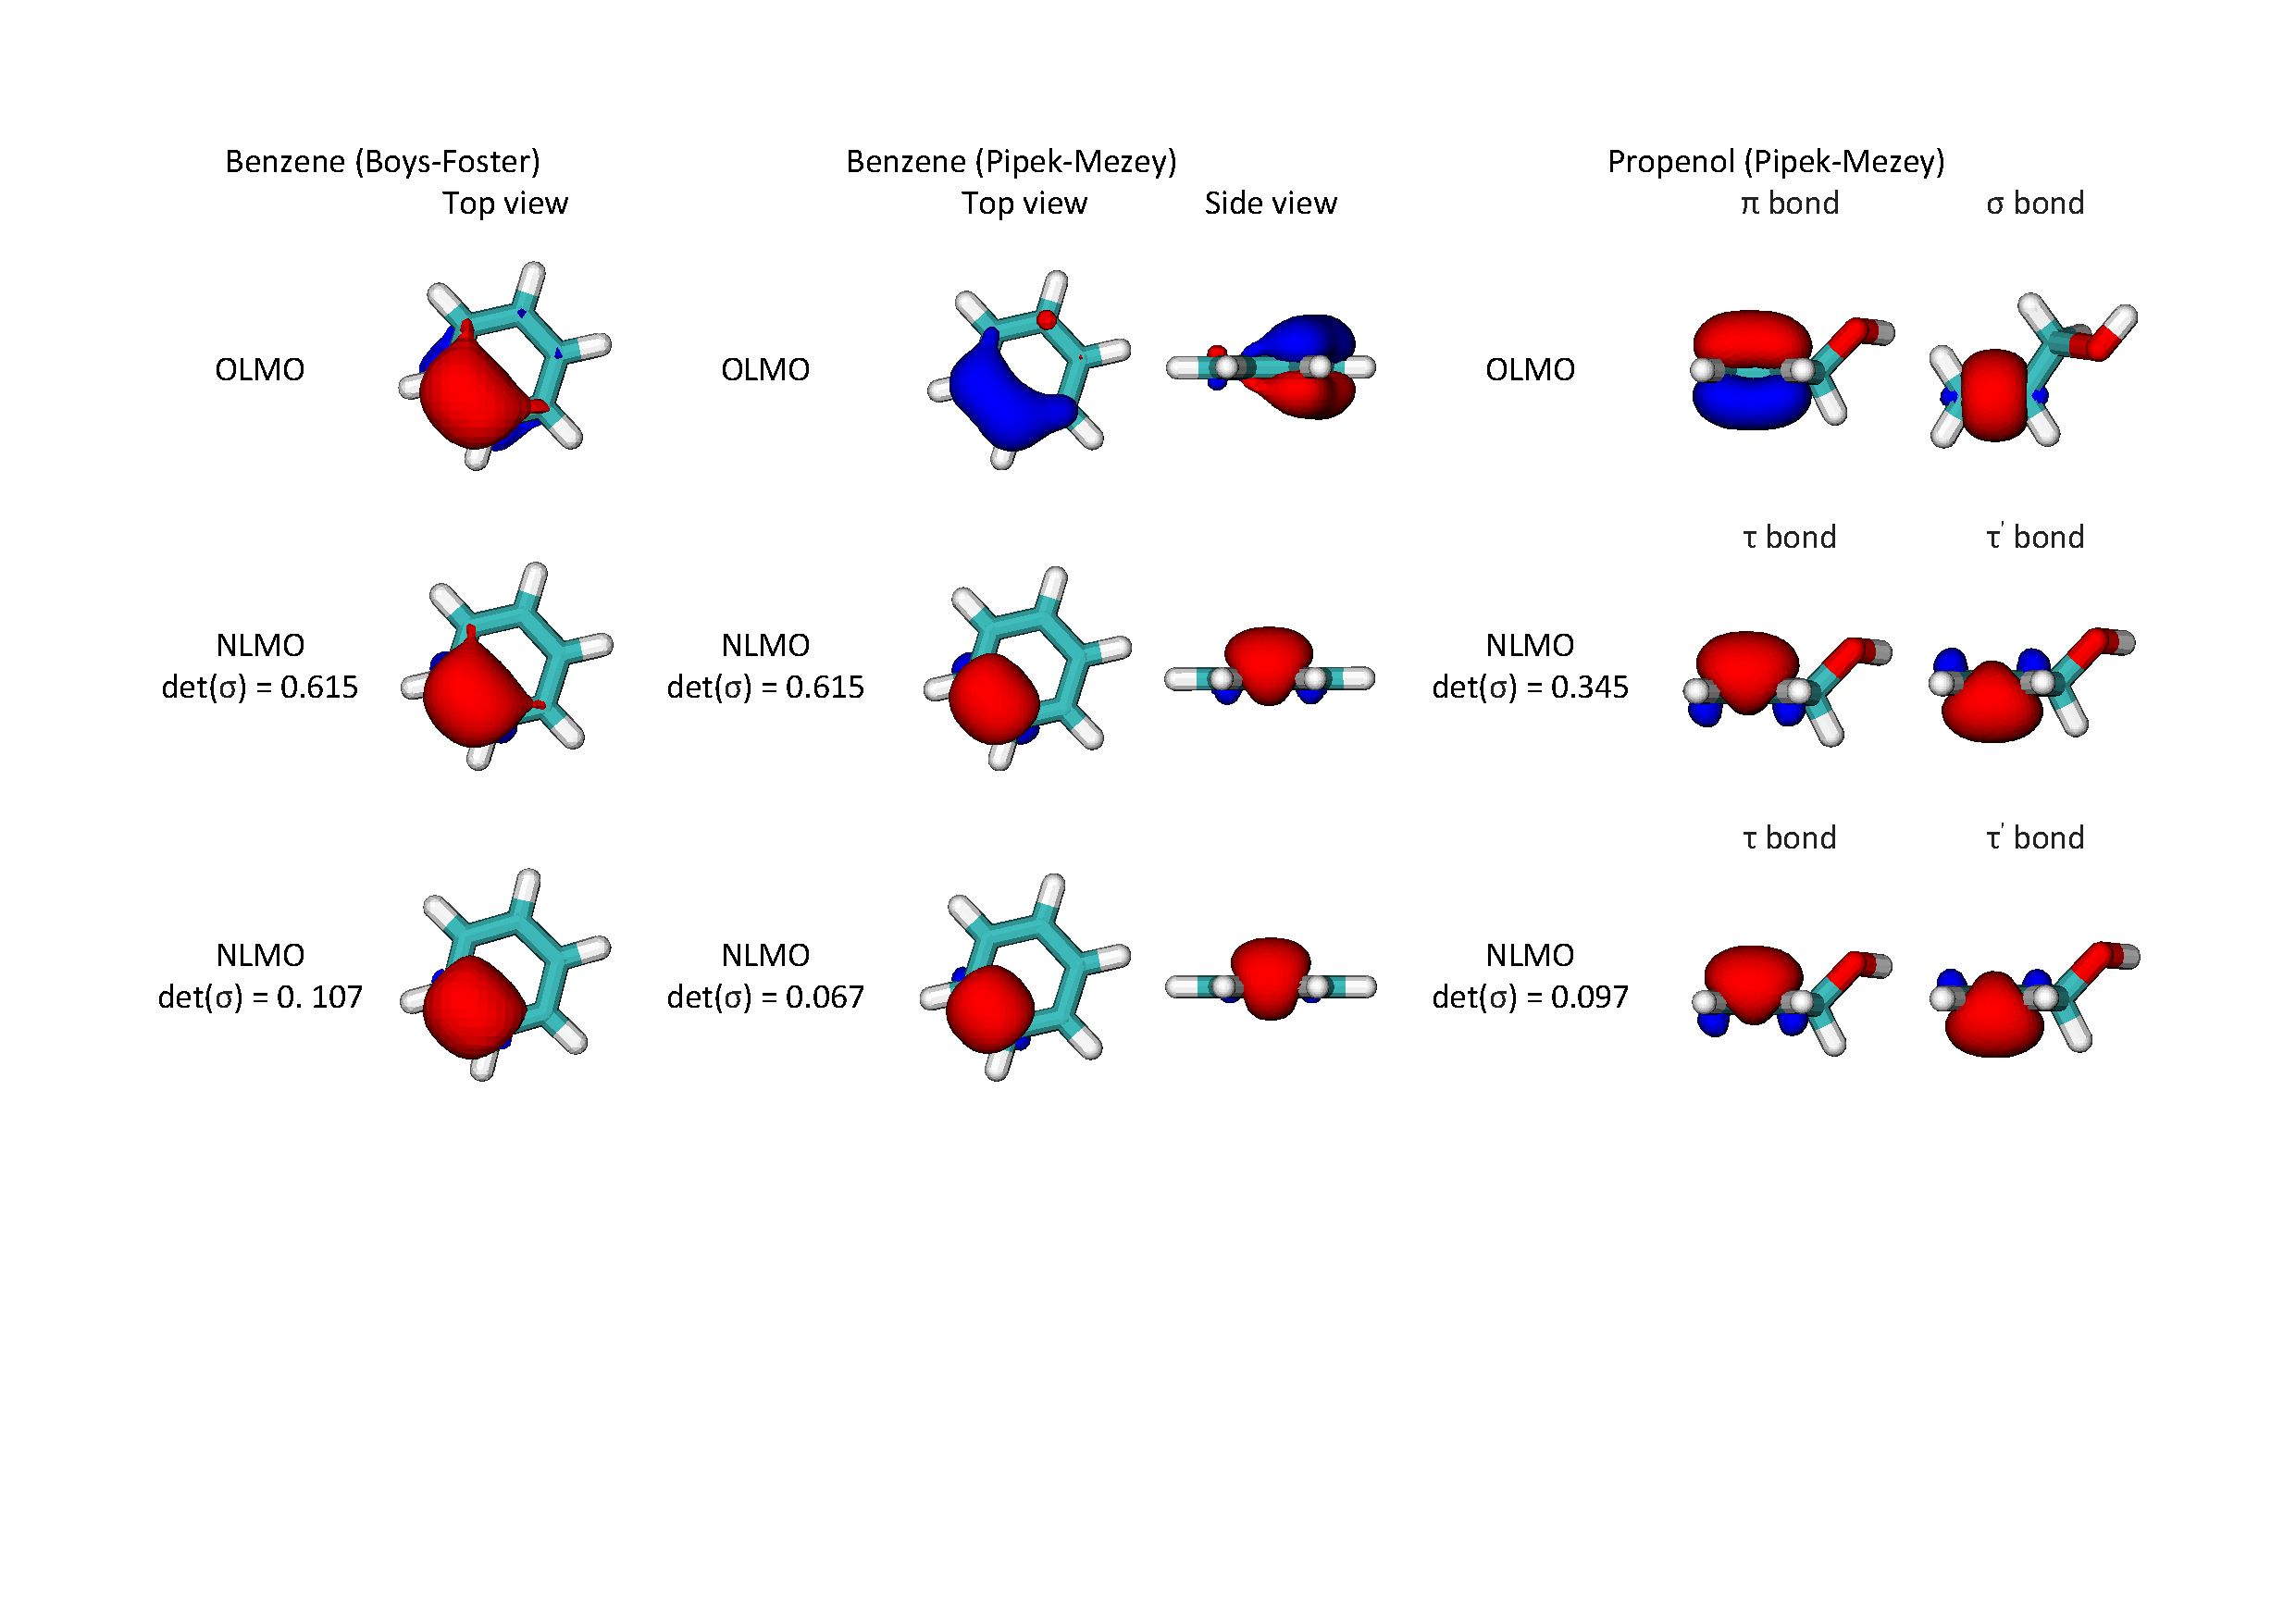
\includegraphics[scale=0.5]{figure_6.pdf}
\caption{Comparison between generated LMOs with Boys-Foster and Pipek-Mezey localization scheme of benzene molecule and A plot of separated $\sigma$ and $\pi$ bonds of OLMOs and mixed $\tau$ and $\tau'$ bonds of NLMOs under Pipek-Mezey scheme. (isosurface value equals to  0.05~a.u.)}
\label{fig:pipek}
\end{figure*}

Although the obtained NLMOs are more localized than the OLMOs in terms of the value of localization functional, we still don't know the the actual shape difference between them.
To show the spatial distribution difference of corresponding NLMO and OLMO, we print out several orbitals for visual comparison.
Figure~\ref{fig:boro} and Figure~\ref{fig:graphene} are a few NLMOs and OLMOs obtained from our tests.
Figure~\ref{fig:boro} describes the NLMOs~(top) and OLMOs~(below) of carbon atoms covalent bond for carborane~(C$_2$B$_{10}$H$_{12}$) molecule.
The obtained NLMOs and OLMOs  are completely equivalent to each other and to the CMOs in their representation of the electronic structure.
The Previous study has proved that two adjacent C atoms form four 3c2e~(3 center 2 electron) B–C–B bonds and a classical C–C bond in ortho-carborane molecule\cite{melichar2018systematic}.
It can be seen from the Figure~\ref{fig:boro} that both OLMO and NLMO can well present the complicated bonding pattern in carborane system and the  prerequisites are no longer needed when generating NLMOs.
The overall shape of the corresponding OLMOs and NLMOs are extremely same, but the OLMOs occupy more space compared with the NLMOs in terms of the orthogonalization tail, which indicates the NLMOs are more compact than the OLMOs.
We also noticed the main lobe~(mark as red in the figure) of the NLMOs is larger than that of OLMOs, which also has been reported by Yang et al~\cite{liu2000nonorthogonal}.
This interesting observation is simply because of the normalization condition.
Since the NLMOs have less space occupation and smaller orthogonalization tails, the main lobes should have relative larger sizes.
The study on carborane system have shown that our new approach successfully avoid using the cumbersome pre-determination and suspicious "chemical intuition" to describe the bonding pattern in the complicated and uncharted systems.

Figure~\ref{fig:graphene} reports two NLMOs (upper panel ) and OLMOs (lower panel), respectively, one for C-C $\sigma$ bond~(second column) and the other for $\pi$ bond~(third and forth column) in the periodic graphene system.
The $\sigma$ bond can be well reproduced by both of the OLMO and NLMO, while both of the MOs fail to present the traditional $\pi$ bond in graphene.
While the generated NLMOs are more localized and  relative reasonably representative of the $\pi$ bond compared with OLMOs due to its more compact property.
But the shape of the NLMO is still more like a mixture between $\sigma$ and $\pi$ bond instead of a pure $\pi$ bond because of the limitation of the Berghold localization functional.
The larger main lobe feature is also confirmed by the C-C $\sigma$ bond in Figure~\ref{fig:graphene}.

To compare the performance of the Pipek-Mezey and Berghold schemes in terms of localization, we also study some of the molecules based on our newly developed NLMOs with Pipek-Mezey localization functional.
The final obtained LMOs listed in the Figure~\ref{fig:pipek} are no longer restricted to NLMOs by increasing the final determinant cutoff up to 0.99 during optimization.
According to the first row of Figure~\ref{fig:pipek}, the generated OLMOs, which which describes the $\pi$ bond in benzene molecule and perfectly separated $\sigma$ and $\pi$ bond in propenol molecule, preserve the $\sigma$ and $\pi$ separation property in OLMOs.
With the final determinants decreasing and the LMOs becoming more and more nonorthogonal, we surprisingly noticed that the property of $\sigma$ and $\pi$ separation of Pipek-Mezey scheme is no longer satisfied.
The NLMO described $\pi$ bond becomes more compact and tend to generate the $\tau$ bond by mixing with $\sigma$ bond in the benzene molecule.
The first two columns of Figure~\ref{fig:pipek} illustrate the comparison between Berghold and Pipek-Mezey localizaiton scheme.
Even though the failure of $\sigma$-$\pi$ separation when generating NLMOs based on the Pipek-Mezey scheme, we still notice that the generated NLMOs with Pipek-Mezey scheme are  more localized and have better representative of bonding pattern compared with those obtained by Berghold scheme.

\begin{equation} \label{eq:pipek-tau}
\begin{split}
\ket{\tau} = 2^{-1/2}\left(\ket{\sigma} + \ket{\pi}\right)\\
\ket{\tau'} = 2^{-1/2}\left(\ket{\sigma} - \ket{\pi}\right)\\
\Omega_L(\mathbf{\sigma}) + \Omega_L(\mathbf{\pi}) < \Omega_L(\mathbf{\tau}) + \Omega_L(\mathbf{\tau'})
\end{split}
\end{equation}

\begin{equation} \label{eq:non-ortho-pipek}
\begin{split}
\ket{\tau} = cos\theta\ket{\sigma} + sin\theta\ket{\pi}\\
\ket{\tau'} = cos\theta\ket{\sigma} - sin\theta\ket{\pi}\\
\Omega_L(\mathbf{\sigma}) + \Omega_L(\mathbf{\pi}) \stackrel{?}{<} \Omega_L(\mathbf{\tau}) + \Omega_L(\mathbf{\tau'})
\end{split}
\end{equation}

In the propenol molecule, the $\pi$ and $\sigma$ bonds are tend to generate the $\tau$ and $\tau'$ bonds, which is the almost same result as we obtained in the Berghold scheme.
In the Pipek-Mezey localization scheme, the previous study has proved that the $\sigma$-$\pi$ separtion is always the stable solution compare with the mixed $\tau$ and $\tau'$ bonds for optimum population localized orbitals in Eq.~\ref{eq:pipek-tau}. The expressions of $\ket{\tau}$ and $\ket{tau'}$ of Pipek-Mezay NLMOs scheme (Eq.~\ref{eq:non-ortho-pipek}) are different from the OLMO scheme, which results in the $\pi$ and $\sigma$ separation is no longer more stable solution than the mixed case.
So that the $\sigma$ and $\pi$ seapration can not be maintained in the nonorthogonal otbitals even based on Pipek-Mezey localization functional.

It is well known that OLMOs remain orthogonality tails whose presence is crucial to satisfy the orthogonal condition for OLMOs , while NLMOs, which remove the orthogonalization constrain, tend to get smaller tails and more compact orbitals. 
To illustrate and compare the tail difference between OLMOs and NLMOs, we plot the NLMO and OLMO of decacyclene~(C$_{72}$H$_{24}$) with small isosurface value (0.003~a.u.).
According to the Figure~\ref{fig:NLMOsvsOLMOs} , we can conclude that the thickness of the orthogonality tails is reduced for the localized NLMOs compared to the orthogonal counterpart.
But the orbital locality has not changed a lot by relaxing the localization centres in molecules and periodic systmes as we initially expected.

\begin{figure}[htbp]
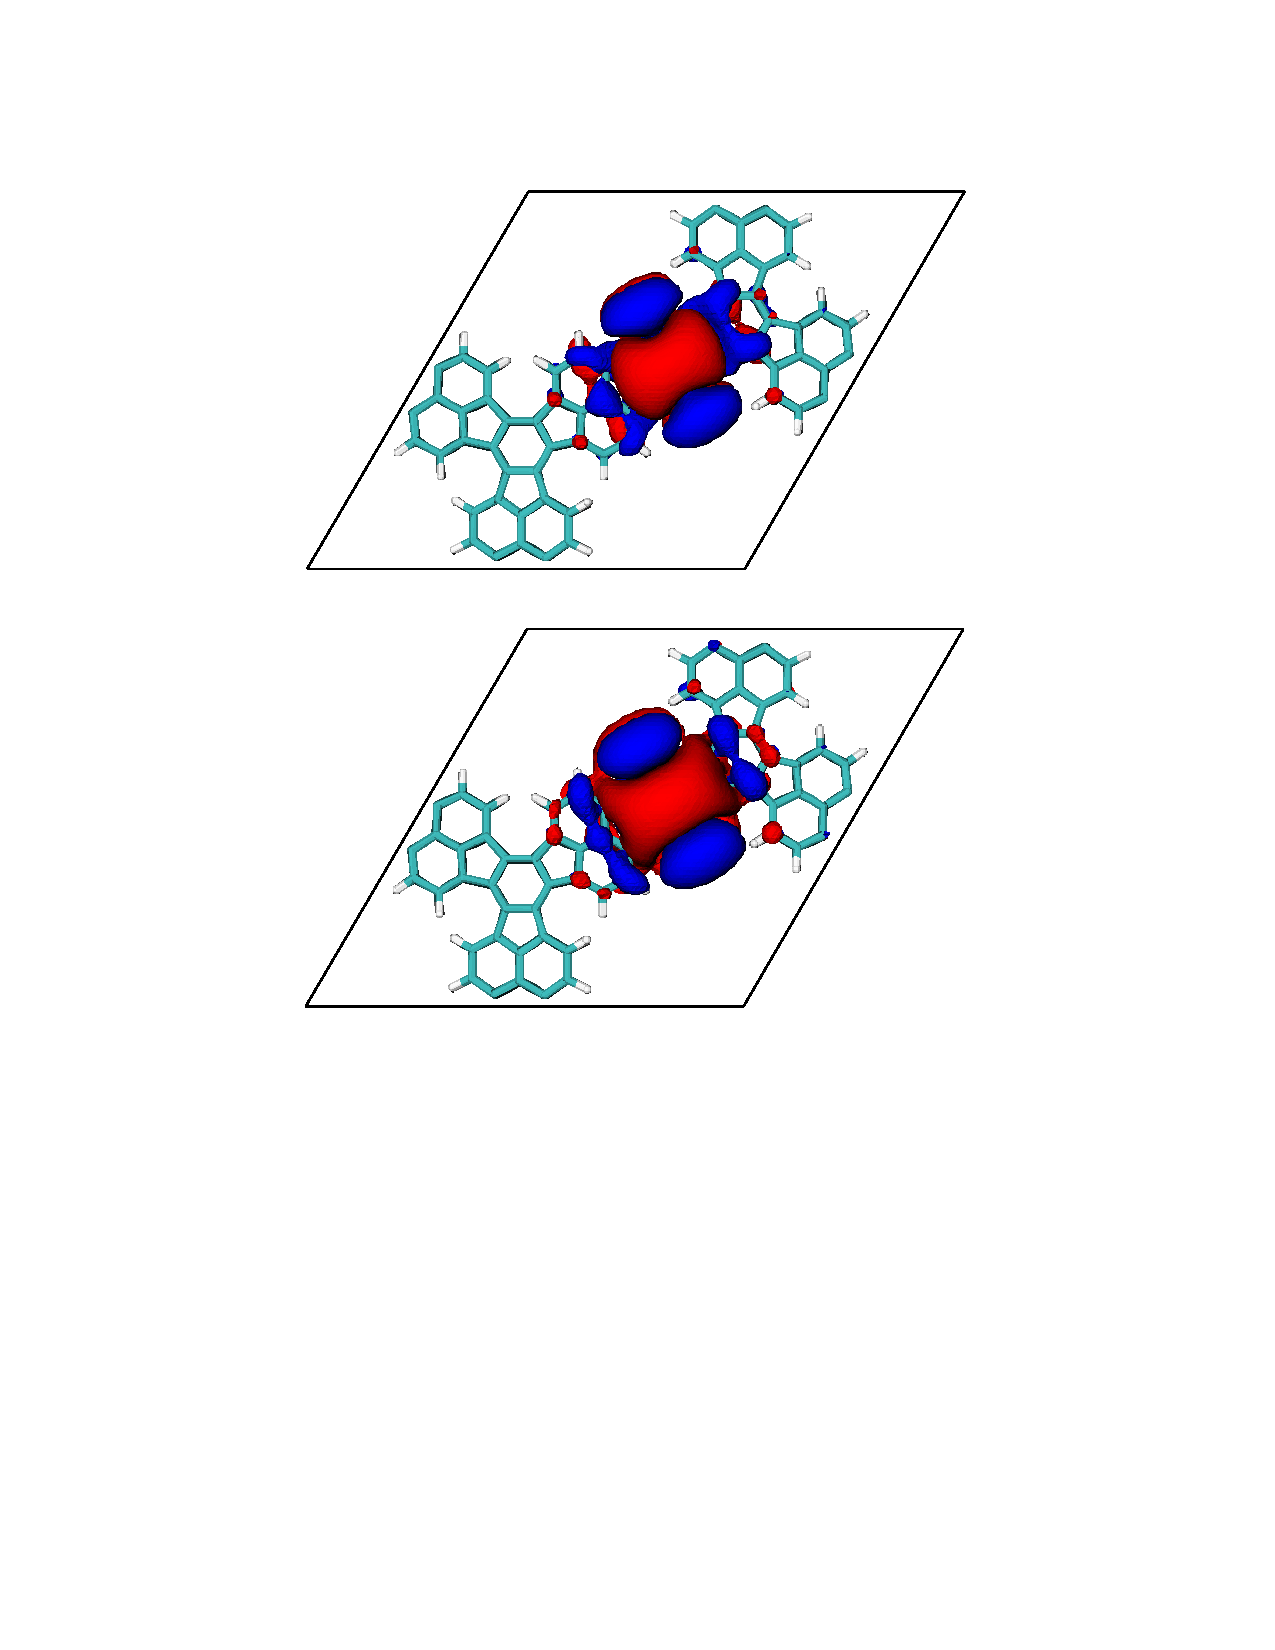
\includegraphics[scale=0.6]{figure_5.pdf} 
  \caption{Comparison of one of the NLMOs (top) and OLMOs (bottom) or a $\pi$ bond in the conjugated decacyclene~(C$_{72}$H$_{24}$) polymer. The isosurface value is set at a relatively low value of 0.002~a.u. to emphasize the tails of the orbitals.)}
\label{fig:NLMOsvsOLMOs}
\end{figure}

In summary, we found that NLMOs are significantly more compact and less tails than corresponding OLMOs based on our newly proposed black-box method. 
We successfully developed a new approach, which minimizes the Berghold or Pipek-Mezey localization functional and automatically self-adjusts penalty function by user specified input, to generate LMOs, especially NLMOs without the need of understanding the bonding patterns in the system or any pre-fixed/defined NLMO centers.
Our results are consistent with the previous study which the NLMOs are around $10\%$ to $30\%$ more localized than the corresponding OLMOs.
As we mentioned before, the Berghold localization functional tends to mox the $\sigma$ and $\pi$ bond during the minimization procedure, so the $\pi$ bond of NLMOs we obtained are slightly different from the traditional bonding pattern.
Further more, we surprisingly noticed that the $\sigma$-$\pi$ separation could not be preserved when generating NLMOs based on Pipek-Mezey localization scheme.
%This problem is possible to be solved if we use Pipek-Mezey~\cite{pipek1989a_fast} localization scheme.
Even though obtained NLMOs with our method have less orthogonality tails compared with conventional OLMOs, we still could observe the significantly existence of tails when using small isosurface value, which means the generated NLMOs are still not nonorthogonal enough to eliminate the tails when using second order localization functional. 
We hope this issue can be solved when applying higher order localization functional.

%RZK: isosurface value -> a.u. use words, not just "isosuface="


%Present localization paths for two systems: simple and challenging. Use $c_P$ values determined by our automatic procedure. Remember that the whole point of creating this method was to make the localization black-box.

%Can we localize virtual orbitals?

%Discuss existing issues: convergence rate, sigma-pi mixing, orthogonalization tails, sparsity of the final coefficients. Mention possible future work to resolve them.

%TODO: Visualize an xyz file with localization centers to make sure NLMOs are physical. Compute the $c_P$ coefficient correctly the equation to minimize the L2 norm of the gradient.

\section{Conclusions}
%RZZK: the algorithm is easy to implement to obtain both OLMOs and NLOMs. In the former case, it does not require to parameterize the unitary transformation.
%RZZK: it is a generalization of the proposed schemes to generate MLWFs. Important for solid state systems.
In this paper, we proposed an unconstrained and generalized black-box method to localize orbitals, especially NLMOs, that automatically determine the centers during the optimization process without any pre-understanding/defined bonding patterns in the system. 
The adjustable penalty function strength allows us to manually regulate the balance between orthogonality and locality of NLMOs.
Our calculations show that the optimization is stable and fast in our most tested systems.
With the help of the penalty function, we did not observe linear dependence issue among generated NLMOs.

Our results, which agree with previous research by Yang et al~\cite{feng2004An_efficient, cui2010efficient}, show that the NLMOs are around $7\%$ and $28\%$ more compact than the corresponding OLMOs and mostly accordance with the traditional chemical bond theory.
Also, we  can conclude that these NOLMOs can be used to present the electronic structure in the completely equivalent to the representations by the OLMOs and CMs.
Moreover, we found that the orthogonal tails are significantly reduced in the NLMOs compared with the OLMOs.
The faster tail decay for nonorthogonal orbitals is due to more degree of freedom are available without using the orthogonality constrains for nonorthogonal orbitals than orthogonal orbitals.

\section{Acknowledgments} 

The research was funded by the Natural Sciences and Engineering Research Council of Canada (NSERC) through Discovery
Grants (RGPIN-2016-0505). The authors are grateful to Compute Canada and, in particular, the McGill HPC Centre for computer time.

\bibliographystyle{apsrev4-1}
\bibliography{NLMOs}

\end{document}
